\documentclass[UTF8]{ctexart}
\usepackage{geometry}
\usepackage{graphicx}
\usepackage[namelimits]{amsmath} %数学公式
\usepackage{amssymb}             %数学公式             %数学字体
\usepackage{mathrsfs} 
\usepackage{txfonts}
\usepackage{float}  %设置图片浮动位置的宏包
\usepackage{subfigure}%插入多图时用子图显示的宏包
\geometry{a4paper,scale=0.80}
\author{左熙辰-2000012103}
\date{}
\title{植物学实验3}
\ctexset{
    section/name= {实验操作}
}
\begin{document}
\maketitle
\section{被子植物营养器官的形态结构}
\subsection*{结果}
\begin{figure}[h]
    \centering
    \subfigure[被子植物根的解剖结构]{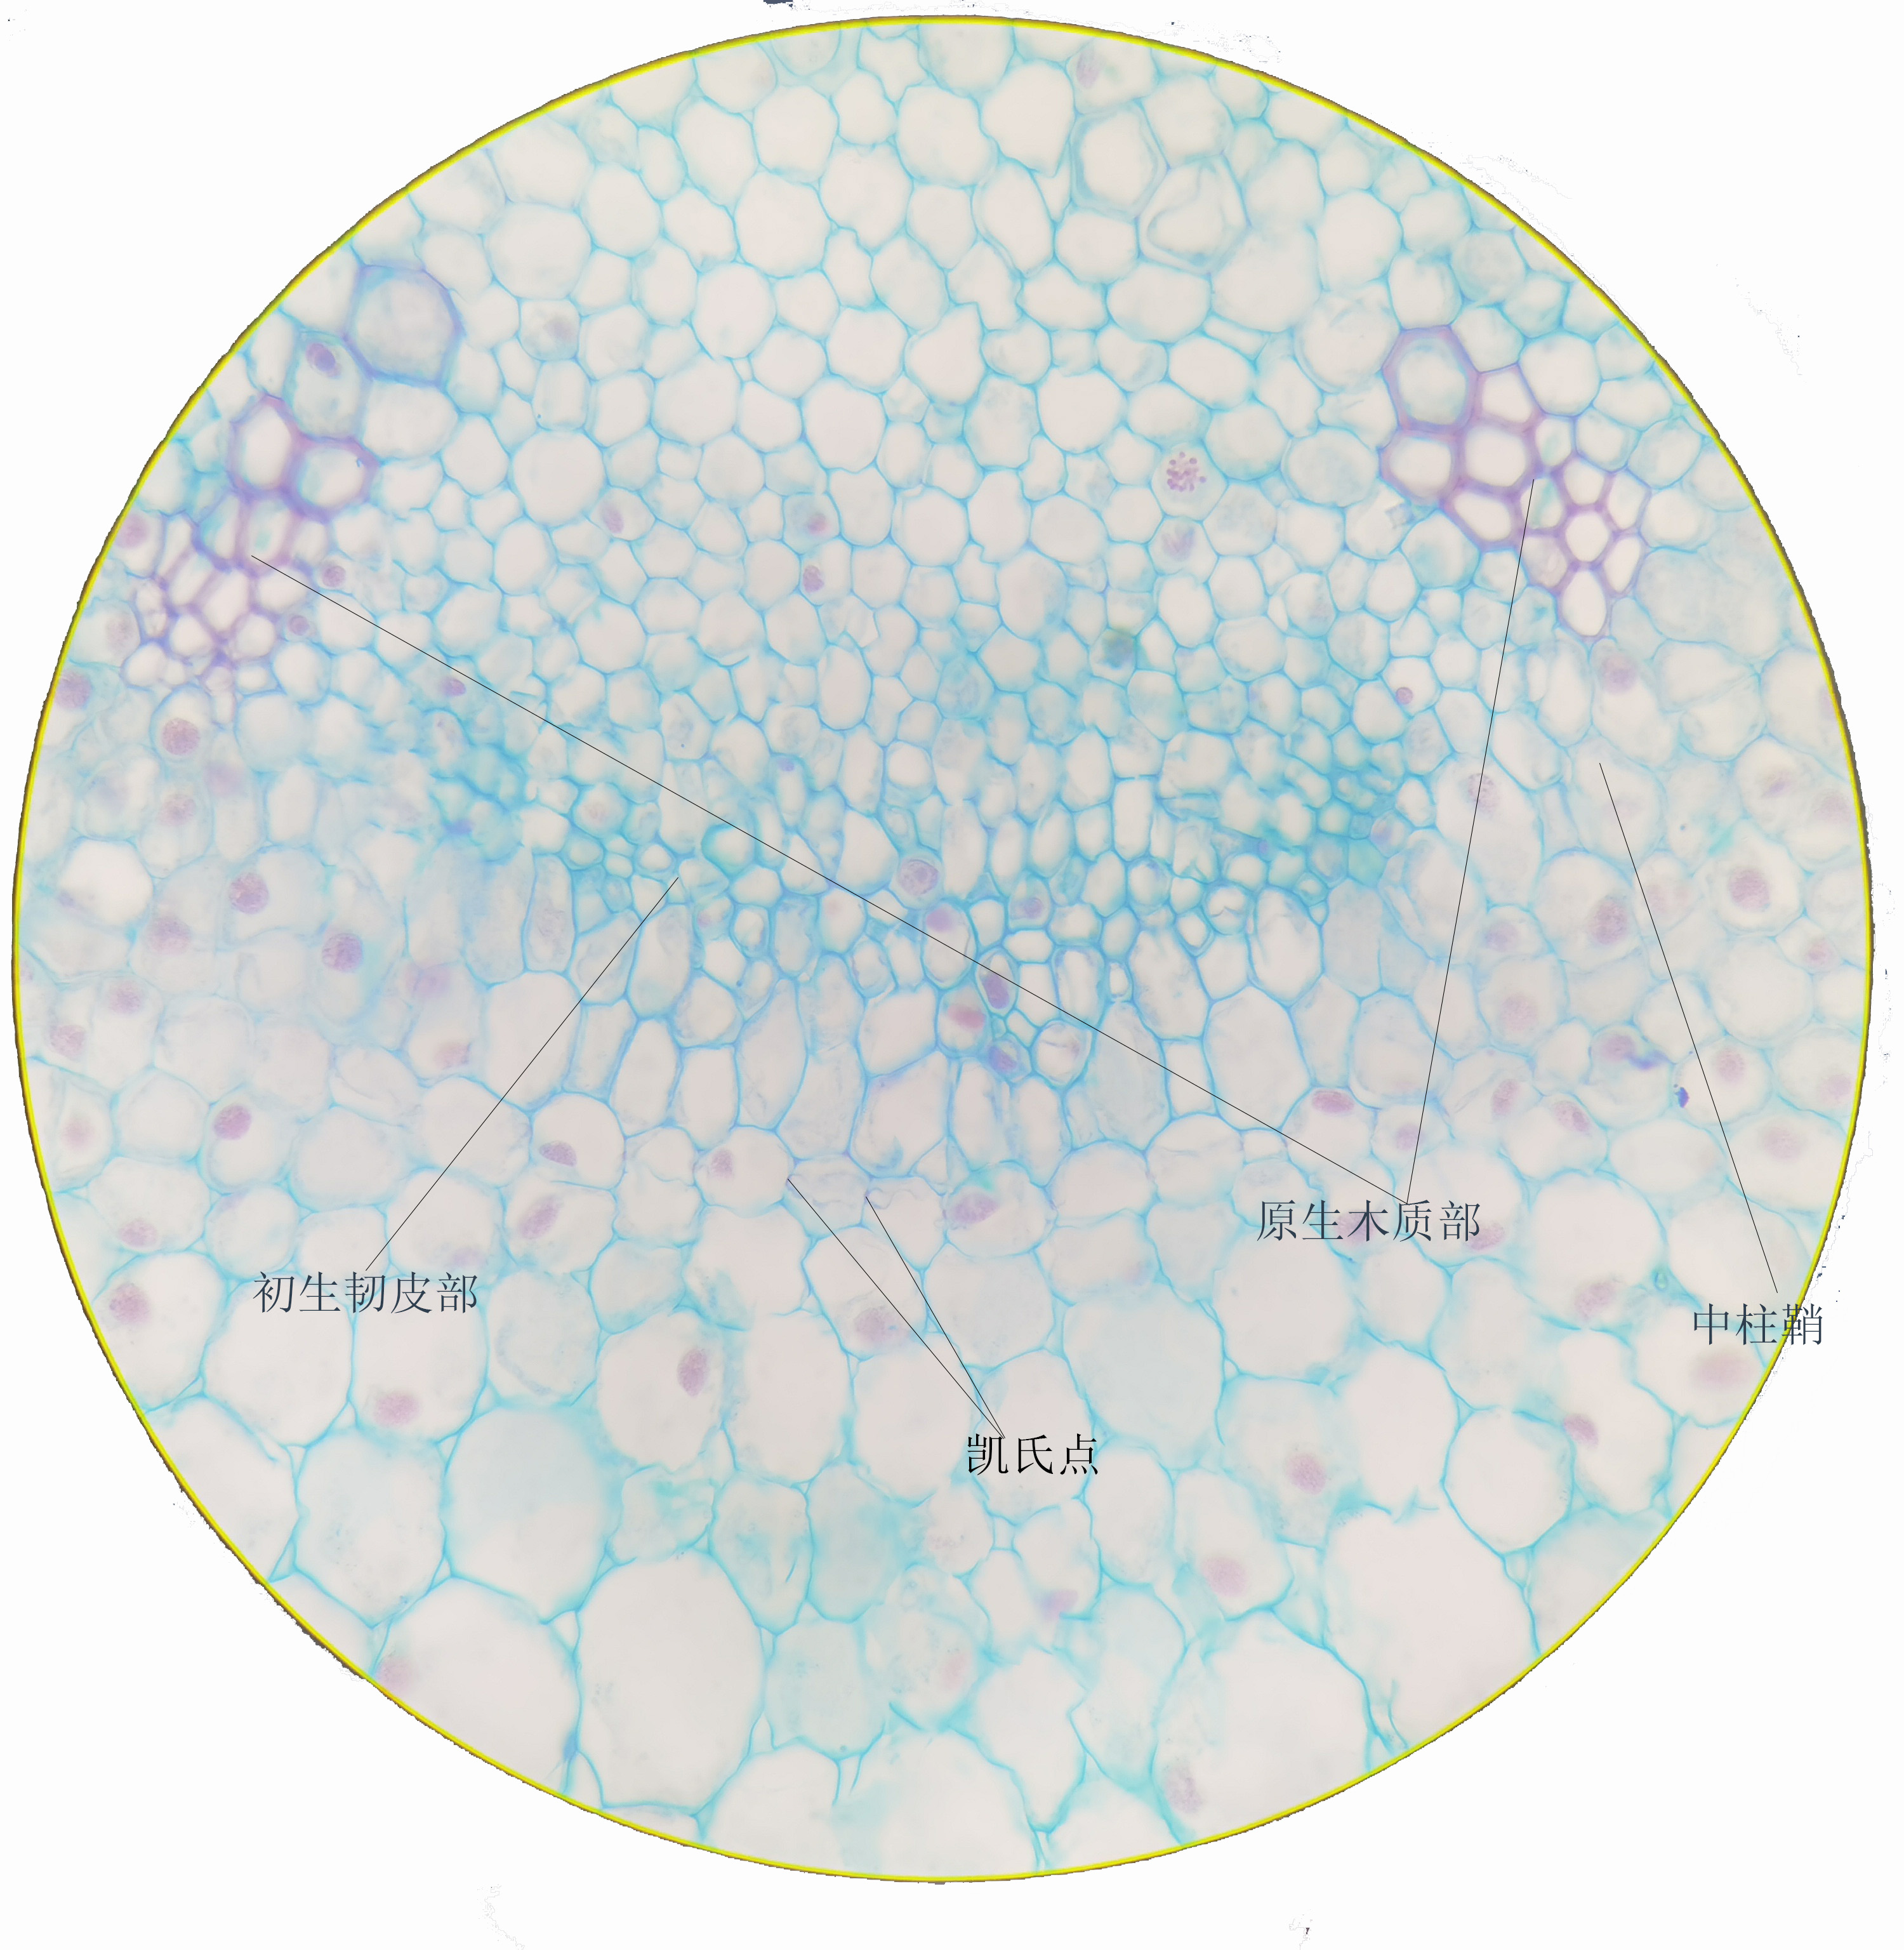
\includegraphics[scale=0.08]{src/botany/IMG_20201202_191549.jpg}\label{gen}}
    \subfigure[被子植物茎的解剖结构]{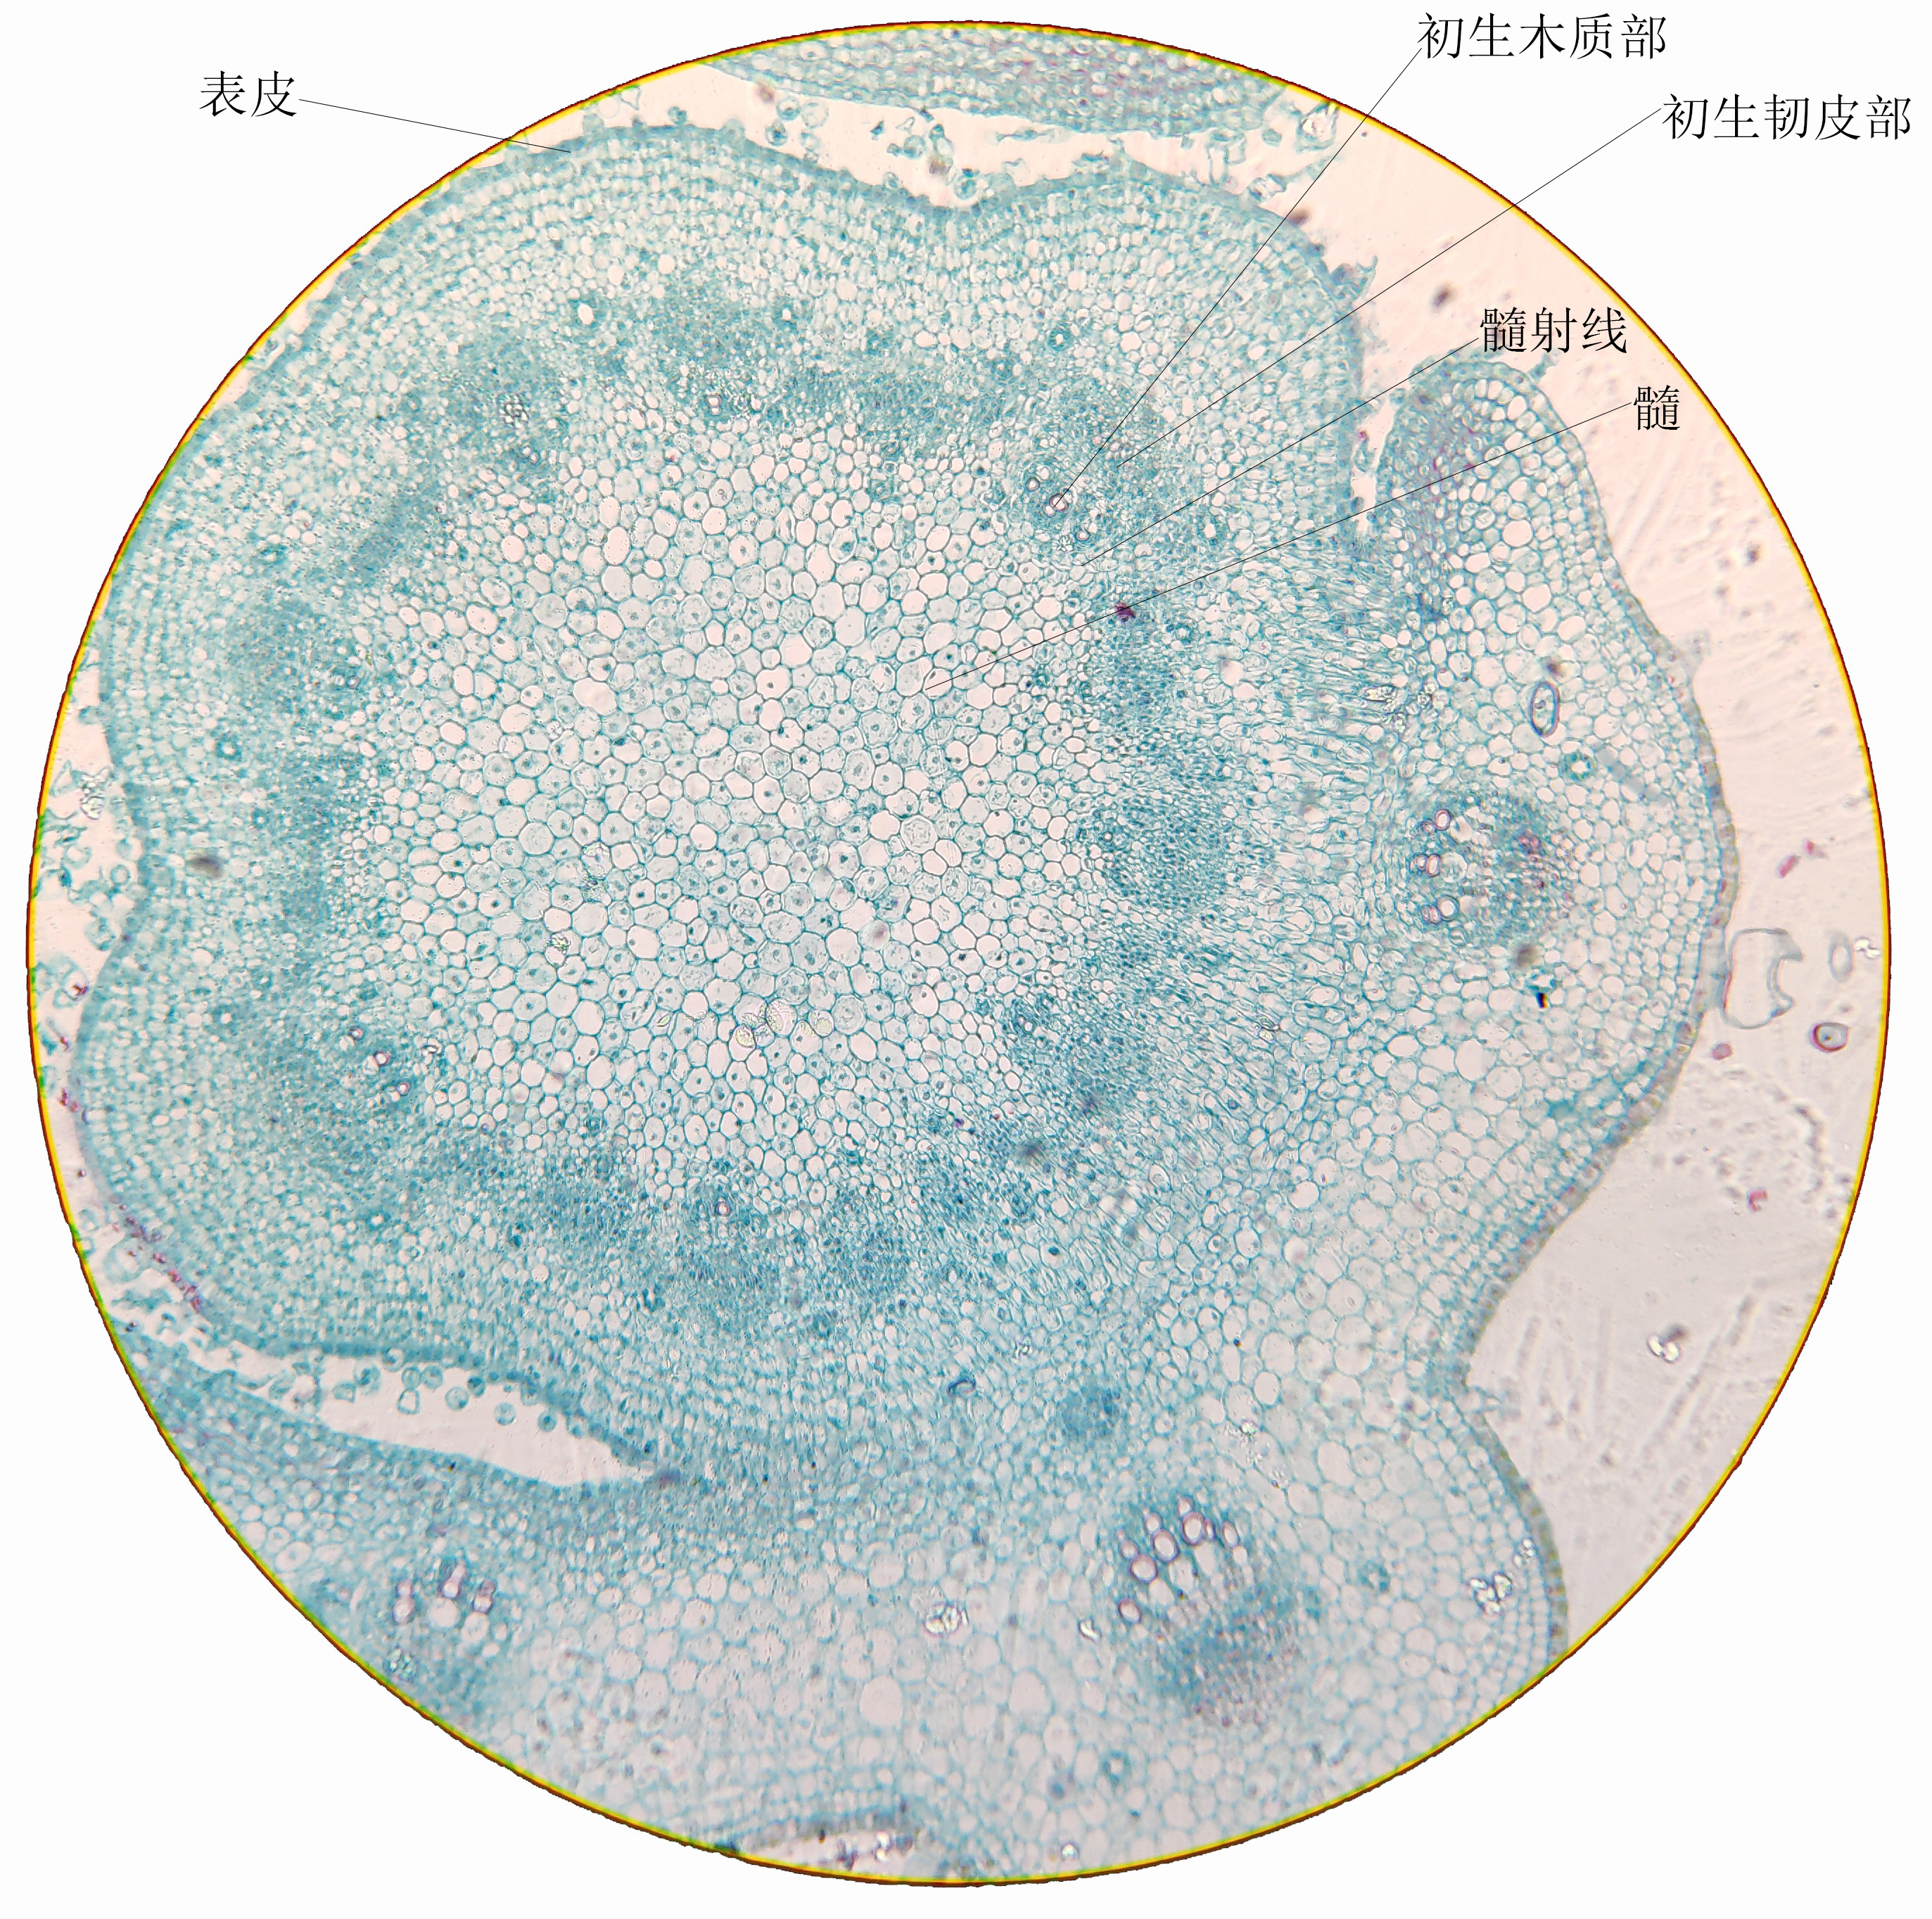
\includegraphics[scale=0.08]{src/botany/微信图片_20201218171831.jpg}\label{jing}}
    \subfigure[水稻叶的结构]{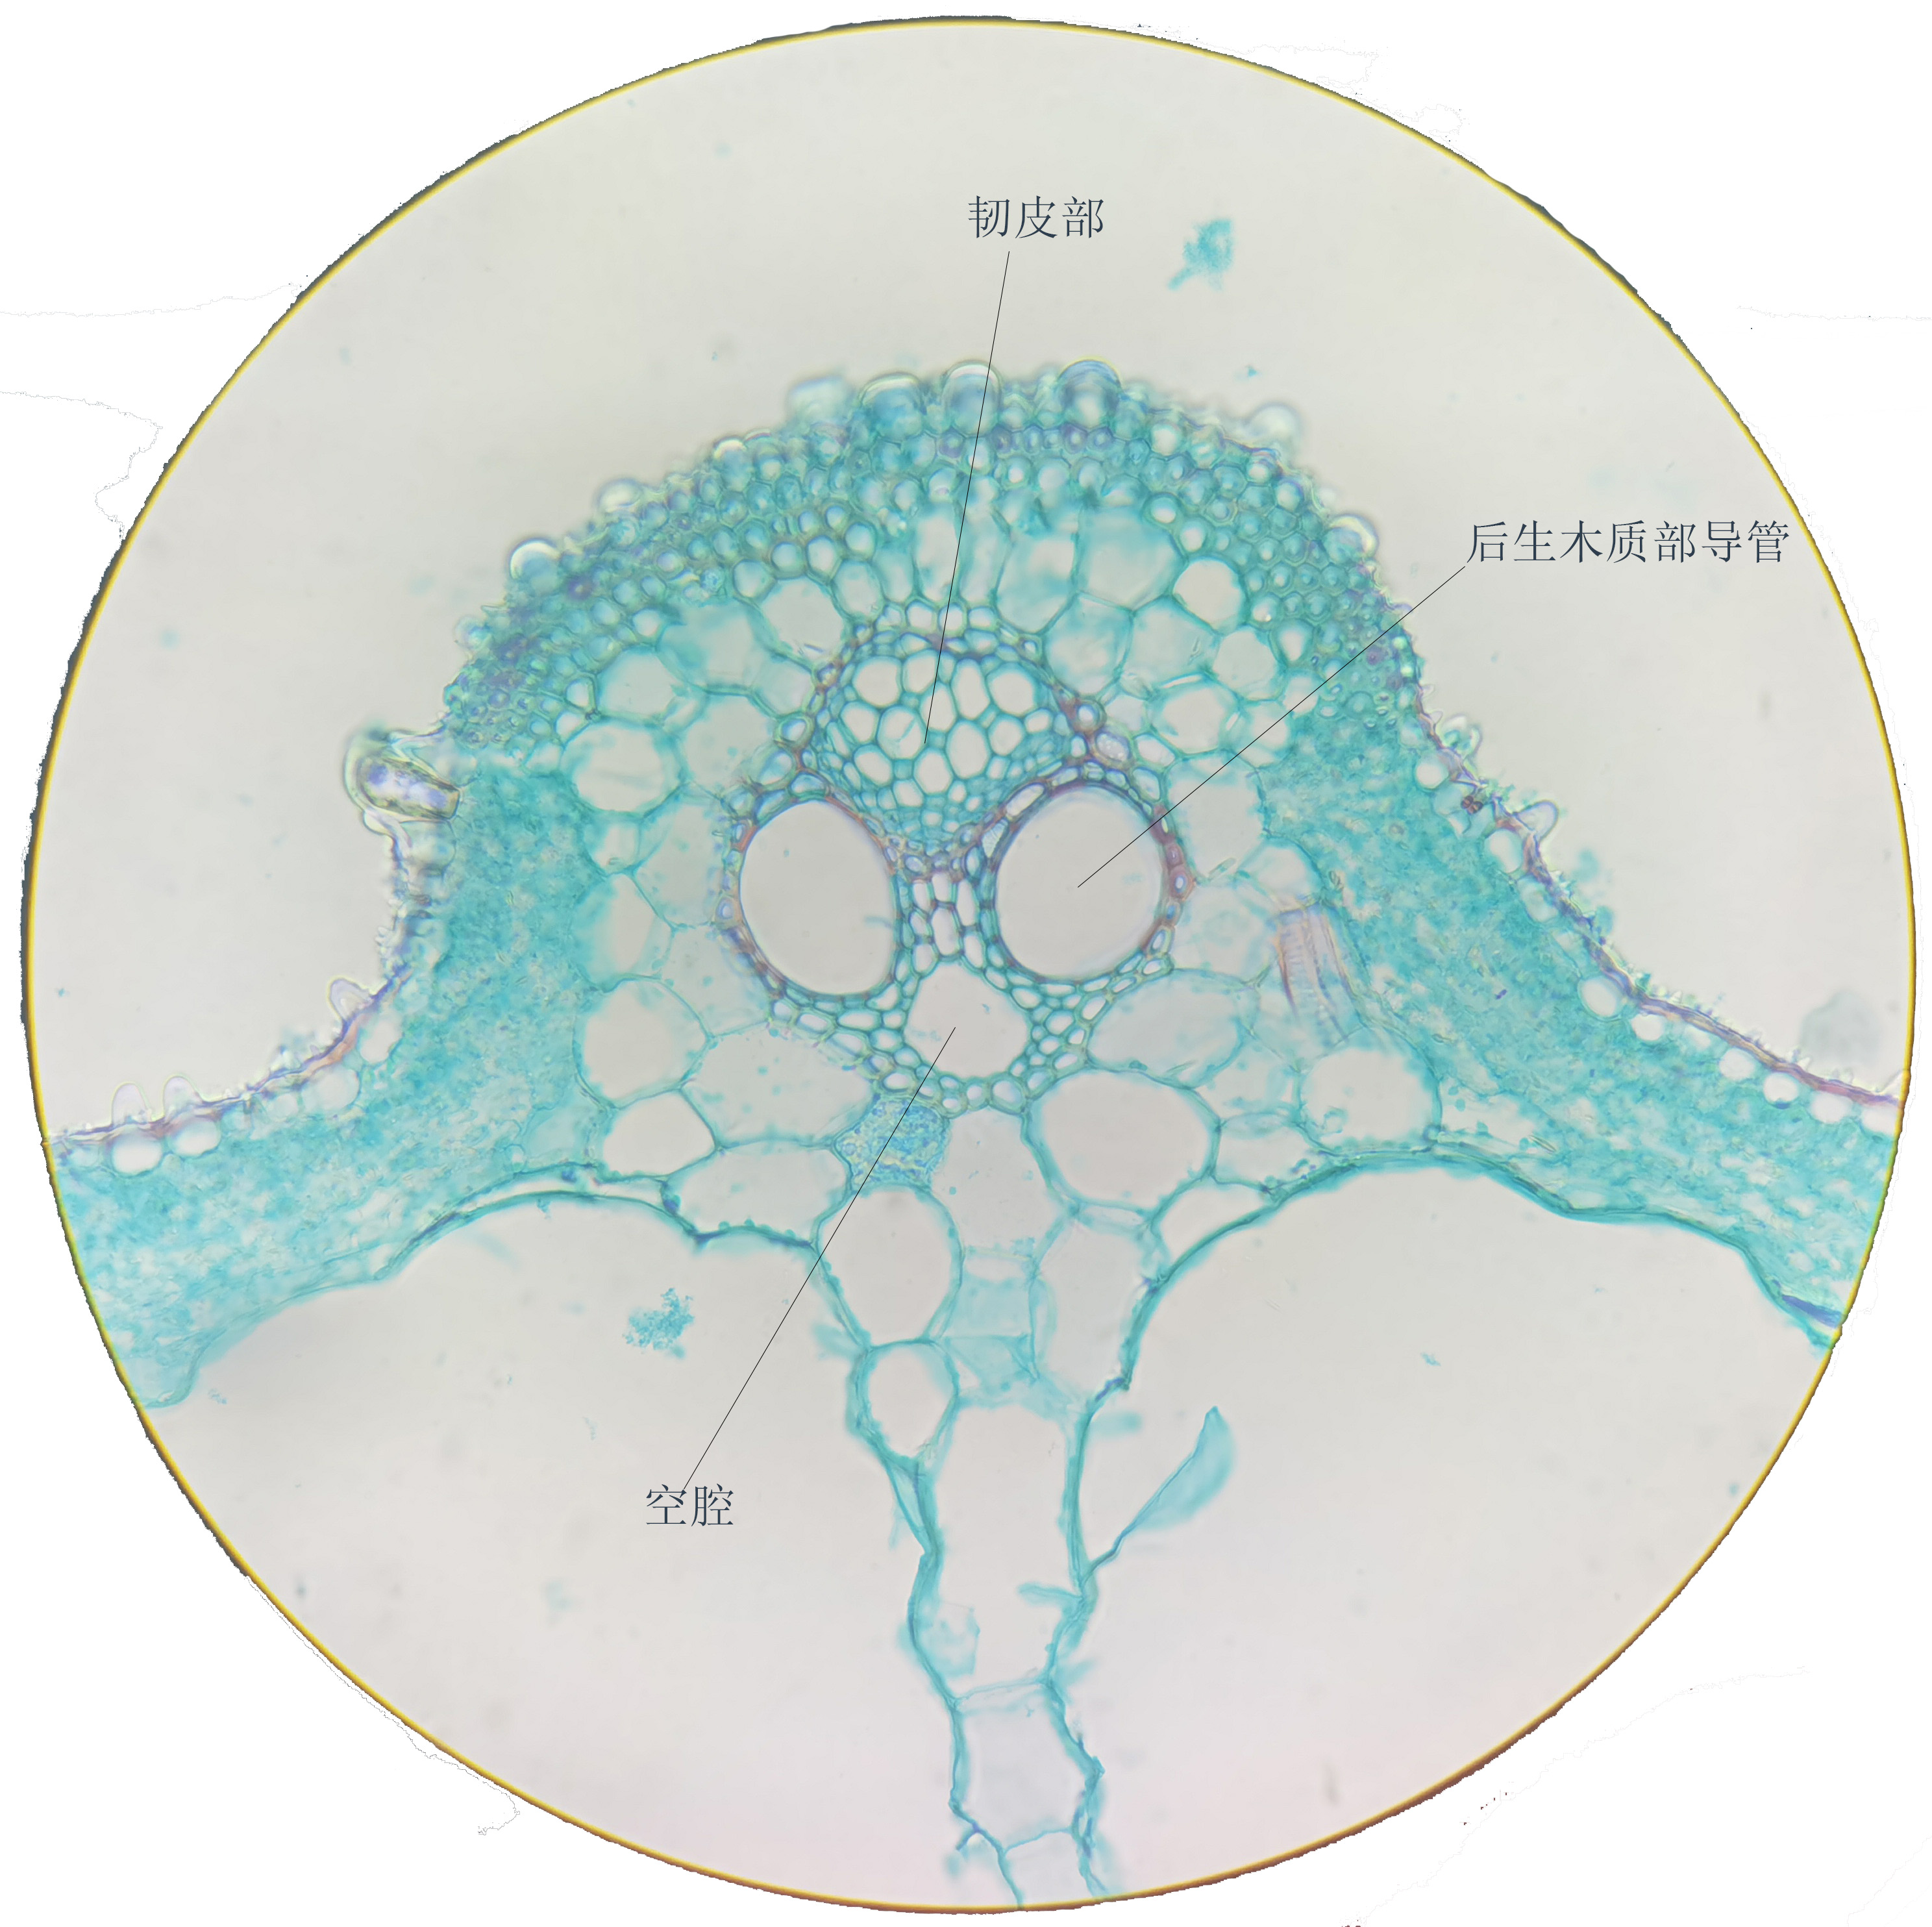
\includegraphics[scale=0.08]{src/botany/IMG_20201202_194703.jpg}\label{shuidao}}
    \subfigure[玉米叶的结构]{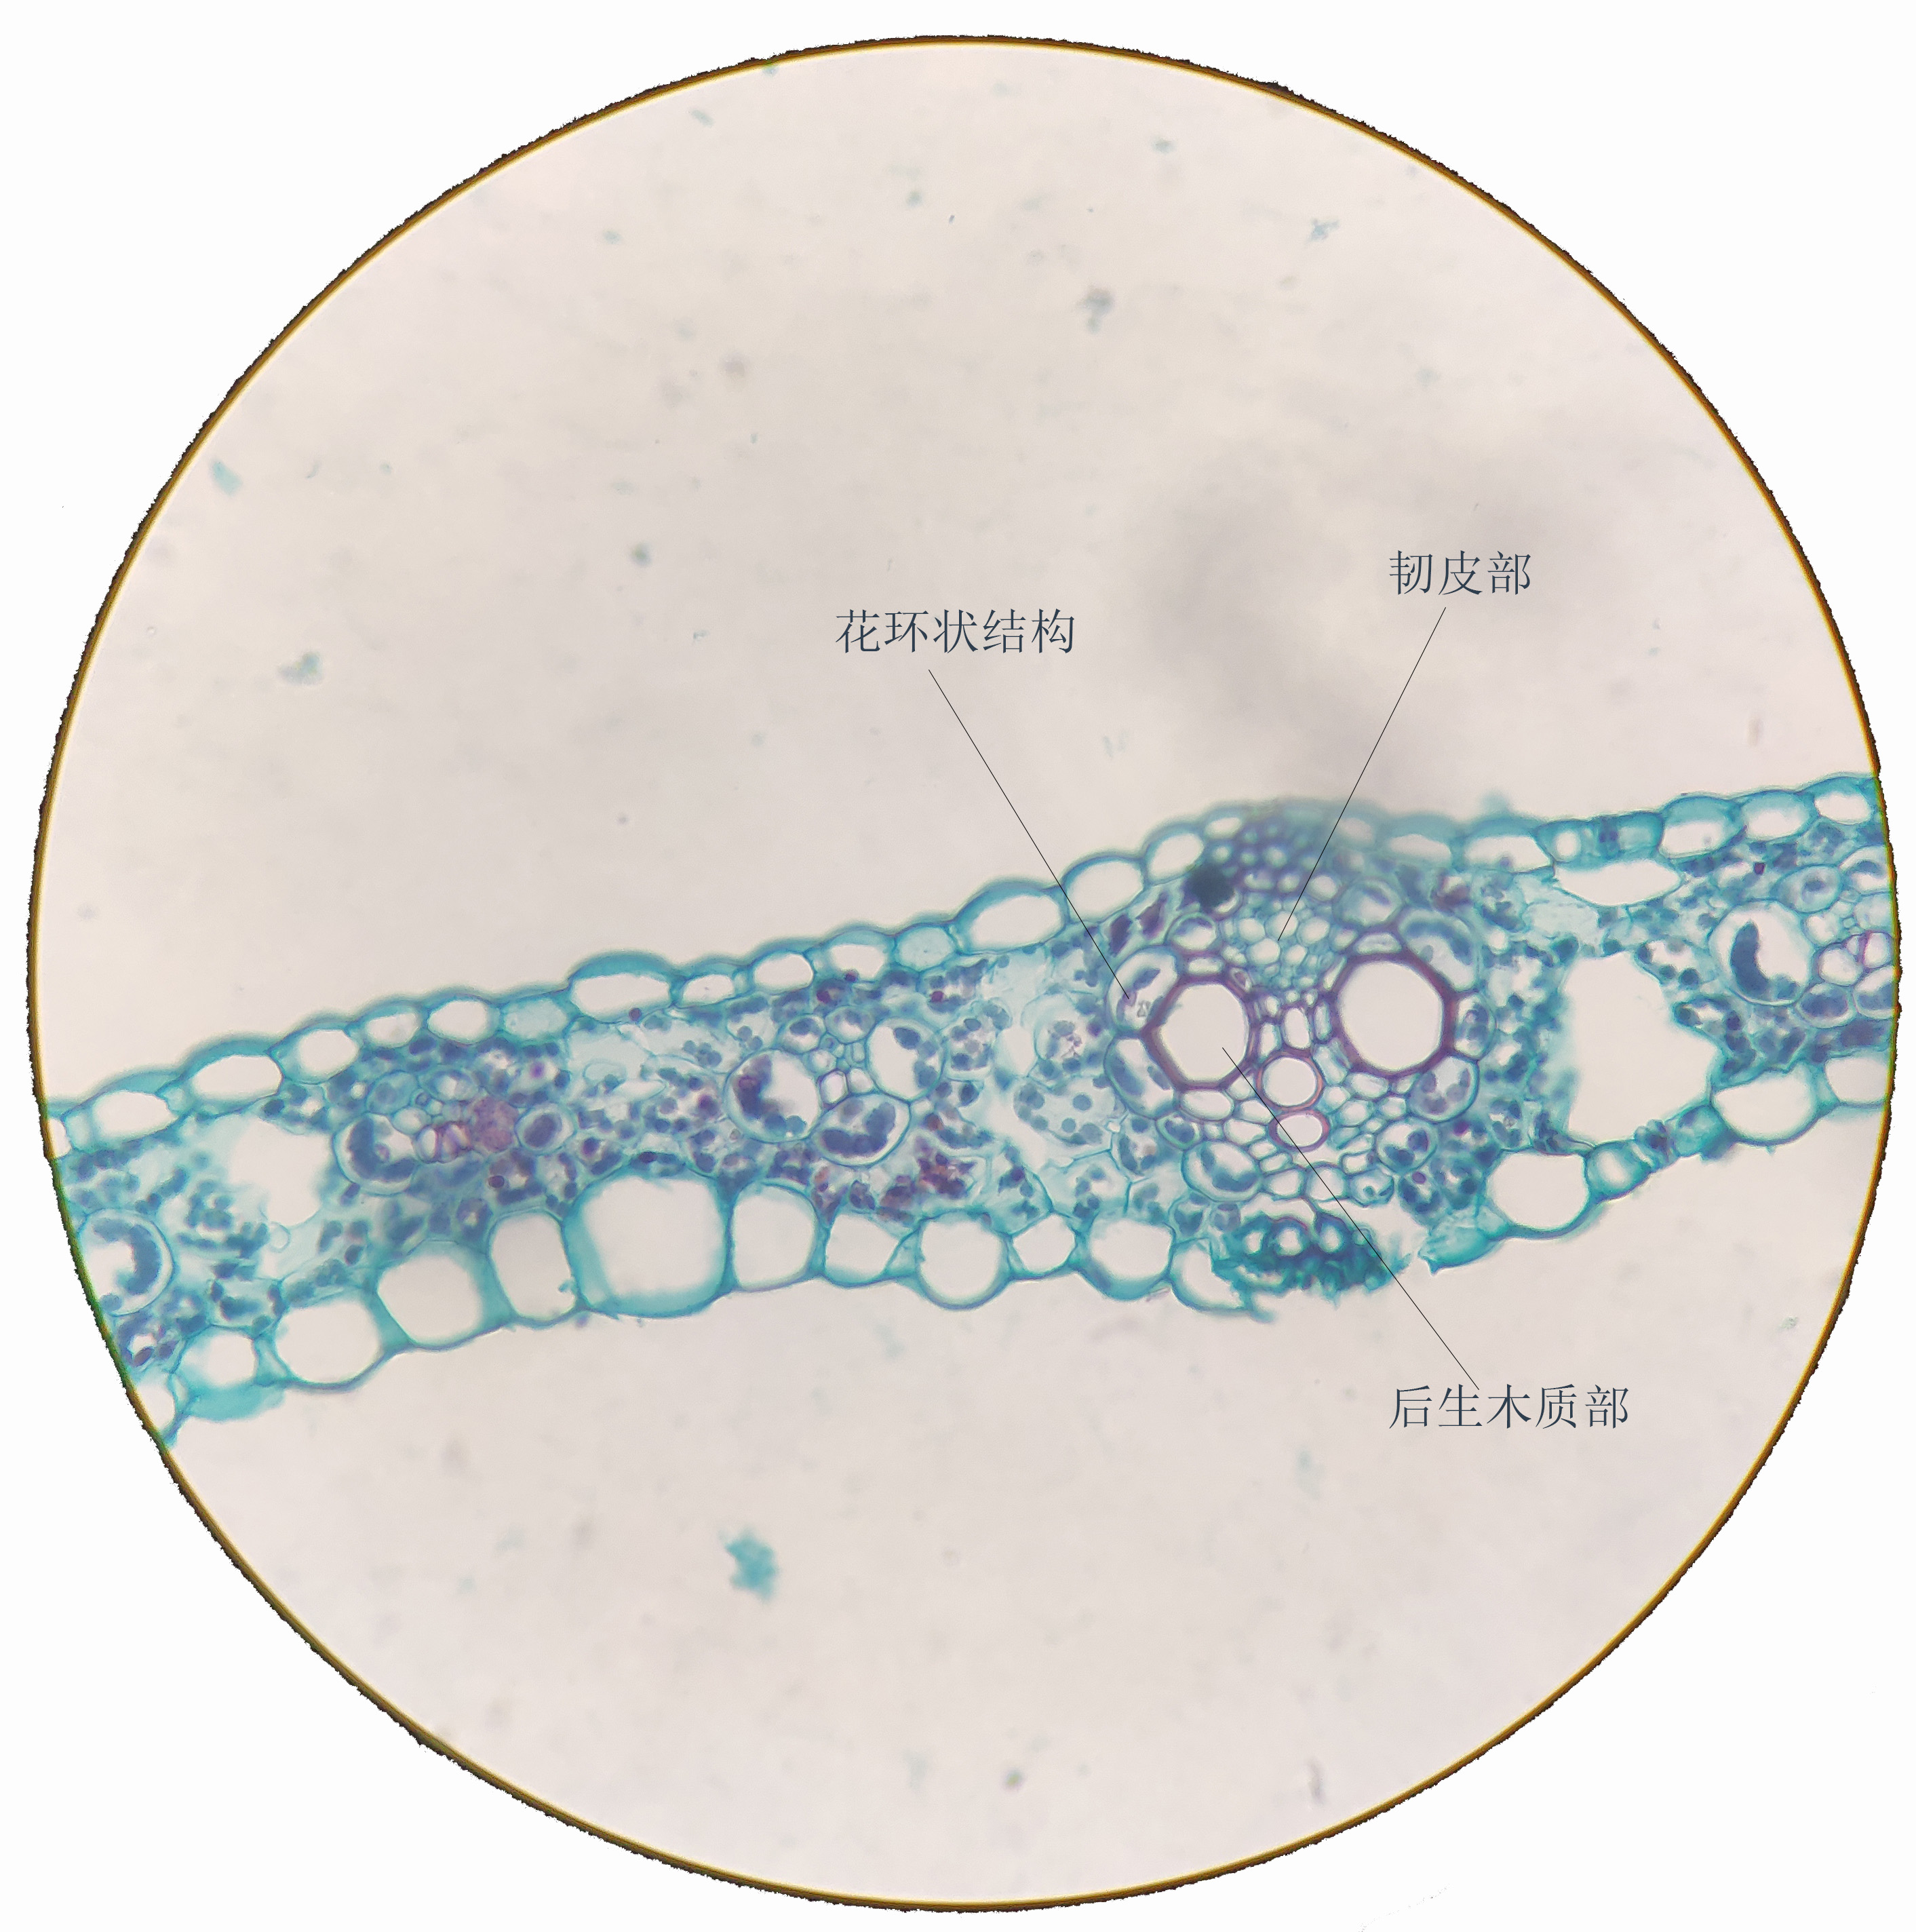
\includegraphics[scale=0.08]{src/botany/微信图片_20201218171818.jpg}\label{yumi}}
    \caption{被子植物营养器官的形态结构}
\end{figure}
    \paragraph*{1.用简图或照片显示被子植物根和茎的解剖结构,并标注出相应的结构名称:}
    \paragraph*{答:}见\ref{gen}和\ref{jing}
    \paragraph*{2.用简图或照片显示水稻、玉米叶的结构,并标注出相应的结构名称。}
    \paragraph*{答:}见\ref{shuidao}和\ref{yumi}
\end{document}